\documentclass{memoir}

\usepackage{hyperref}
\usepackage{graphicx}
\usepackage{tikz}

\usepackage{color}
\definecolor{keyword}{rgb}{0,0,1}		% keywords
\definecolor{comments}{rgb}{0.2,0.5,0.25}	% comments
\definecolor{identifier}{rgb}{0.2,0.2,0.2}	% identifiers

\usepackage{listings}

\lstset{
	basicstyle = \ttfamily ,% Font type
	numberstyle = \small, 	% Font style of numbers
	numbersep = 7pt, 		% Space between line number and code
	keywordstyle = \color{keyword},	% style for keywords
	commentstyle = \color{comments}, % style for comments
	stringstyle = \color{identifier}, 
	breaklines = true,		% Automatic line breaking
	tabsize = 4,				% number of spaces for TAB
	captionpos = b,
	frame = single
}


\title{Stocks Specifications}
\author{Jan Veen}

\begin{document}
\maketitle
\frontmatter

\tableofcontents
\listoffigures
\listoftables
\mainmatter

\part{}
\chapter{Bitemporal Data Model}
\pagebreak
\section{Operations}

\subsection{Current Insert}

\begin{itemize}
\item 1: \texttt{currentInsert("Glass")}
\end{itemize}

Table content after all operations:\\

\begin{tabular}{c  | c | c | c | c}
	vt start & vt end & tt start & tt end & value\\\hline
	1 & i & 1 & i & Glas
\end{tabular}
\\\\
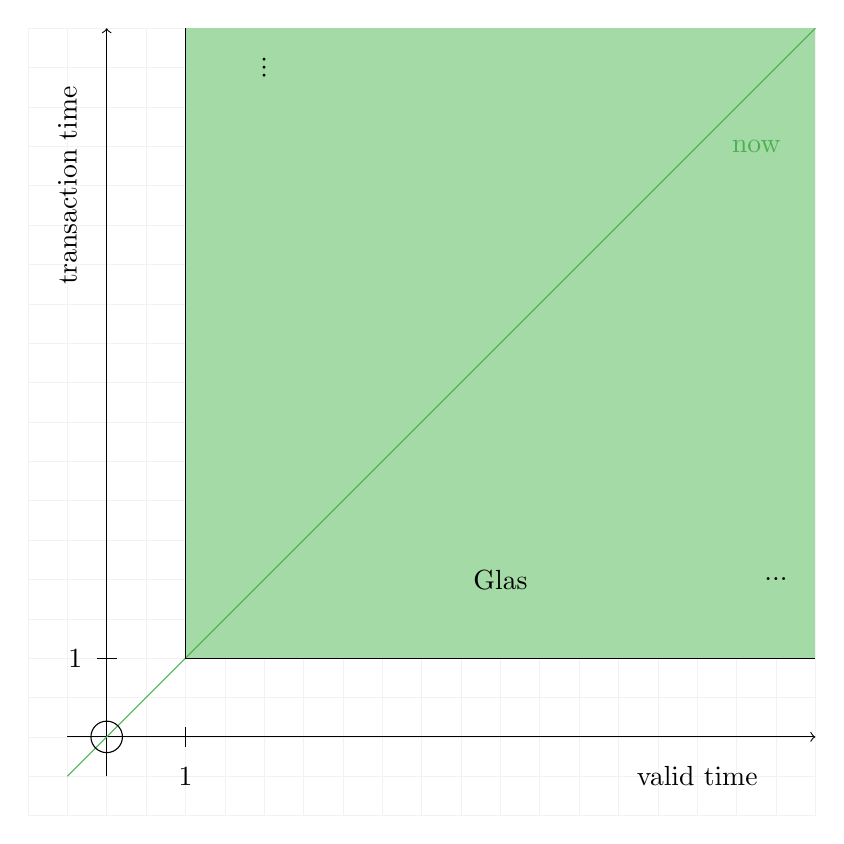
\begin{tikzpicture}
	\definecolor{brightgray}{rgb}{0.95, 0.95, 0.95}
	\definecolor{darkgreen}{RGB}{76, 175, 80}
	\definecolor{content1}{RGB}{163,218,165}
	\definecolor{content2}{RGB}{118,188,121}
	
	\draw[step=.5cm,brightgray,very thin] (-1,-1) grid (9,9);
	\draw[->](-0.5, 0) -- (9,0);
	\draw[->](0, -0.5) -- (0, 9);
	\fill[content1] (1,9) -- (1,1) -- (9,1) -- (9,9);
	
	\draw[darkgreen] (-0.5,-0.5) -- (9,9);
	\draw (0,0) circle [radius=0.2];
	\draw(-0.125, 1) -- (0.125, 1);
	\draw(1,-0.125) -- (1,0.125);
	\draw (1,9) -- (1,1) -- (9,1);
	
	\draw (-0.4, 1) node {1};
	\draw (1, -0.5) node {1};
	\draw (5,2) node {Glas};
	\draw[darkgreen](8.25,7.5) node {now};
	\draw(8.5, 2) node {...};
	\draw(2, 8.5) node [rotate=90] {...};
	\draw (7.5, -0.5) node {valid time};
	\draw (-0.5, 7) node [rotate=90] {transaction time};
	
\end{tikzpicture}

\subsection{Current Update}

\begin{itemize}
	\item 1: \texttt{currentInsert("Glass")}
\item 3: \texttt{currentUpdate("Jar")}
\end{itemize}

Table content after all operations:\\

\begin{tabular}{c  | c | c | c | c}
	vt start & vt end & tt start & tt end & value\\\hline
	1 & i & 1 & 3 & Glas \\\hline
	1& 3 & 3 & i & Glas \\\hline
	3 & i & 3 & i & Jar
\end{tabular}
\\\\

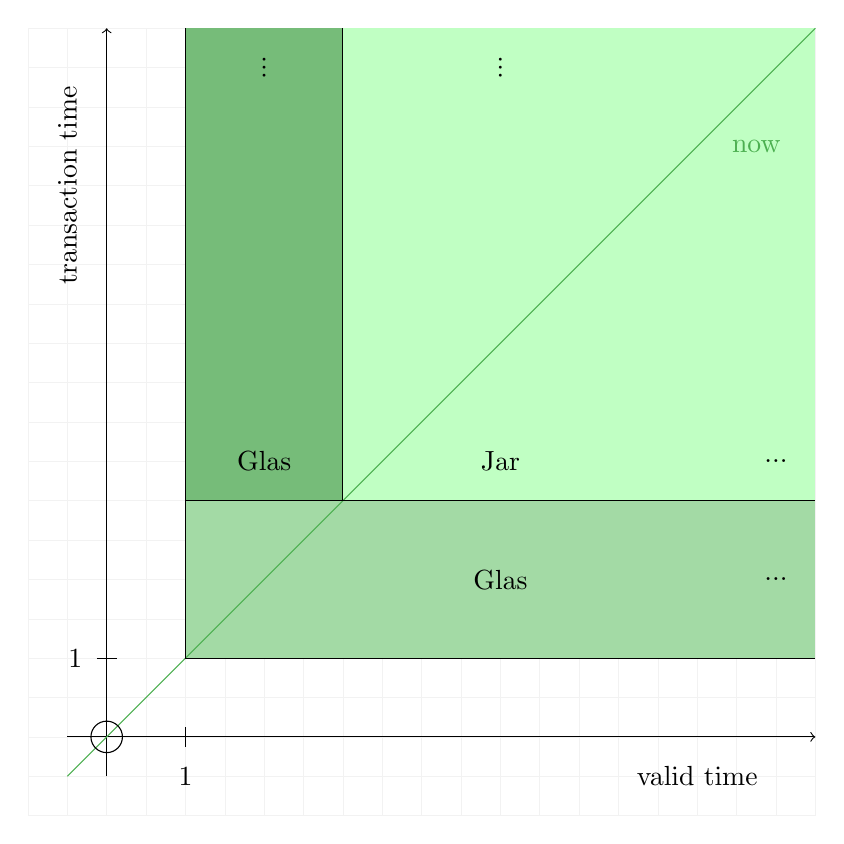
\begin{tikzpicture}
	\definecolor{brightgray}{rgb}{0.95, 0.95, 0.95}
	\definecolor{darkgreen}{RGB}{76, 175, 80}
	\definecolor{content1}{RGB}{163,218,165}
	\definecolor{content2}{RGB}{118,188,121}
	\definecolor{content3}{RGB}{192,255,195}
	
	\draw[step=.5cm,brightgray,very thin] (-1,-1) grid (9,9);
	\draw[->](-0.5, 0) -- (9,0);
	\draw[->](0, -0.5) -- (0, 9);
	\fill[content1] (1,3) -- (1,1) -- (9,1) -- (9,3);
	\fill[content2] (1,3) -- (3,3) -- (3,9) -- (1,9);
	\fill[content3] (3,9) -- (3,3) -- (9,3) -- (9,9);
	
	\draw[darkgreen] (-0.5,-0.5) -- (9,9);
	\draw (0,0) circle [radius=0.2];
	\draw(-0.125, 1) -- (0.125, 1);
	\draw(1,-0.125) -- (1,0.125);
	
	\draw (1,9) -- (1,1) -- (9,1);
	\draw (1,3) -- (3,3) -- (3,9);
	\draw (3,3) -- (9,3);
	
	\draw (-0.4, 1) node {1};
	\draw (1, -0.5) node {1};
	\draw (5,2) node {Glas};
	\draw (2,3.5) node {Glas};
	\draw (5, 3.5) node {Jar};
	\draw[darkgreen](8.25,7.5) node {now};
	\draw(8.5, 2) node {...};
	\draw(2, 8.5) node [rotate=90] {...};
	\draw(8.5, 3.5) node {...};	
	\draw(5, 8.5) node [rotate=90] {...};
	\draw (7.5, -0.5) node {valid time};
	\draw (-0.5, 7) node [rotate=90] {transaction time};
	
\end{tikzpicture}

\subsection{Current Delete}

\begin{itemize}
\item 1: \texttt{currentInsert("Glass")}
\item 3: \texttt{currentUpdate("Jar")}
\item 6: \texttt{currentDelete()}
\end{itemize}


Table content after all operations:\\

\begin{tabular}{c  | c | c | c | c}
	vt start & vt end & tt start & tt end & value\\\hline
	1 & i & 1 & 3 & Glas \\\hline
	1& 3 & 3 & i & Glas \\\hline
	3 & i & 3 & 6 & Jar \\\hline
	3 & 6 & 6 & i & Jar
\end{tabular}
\\\\

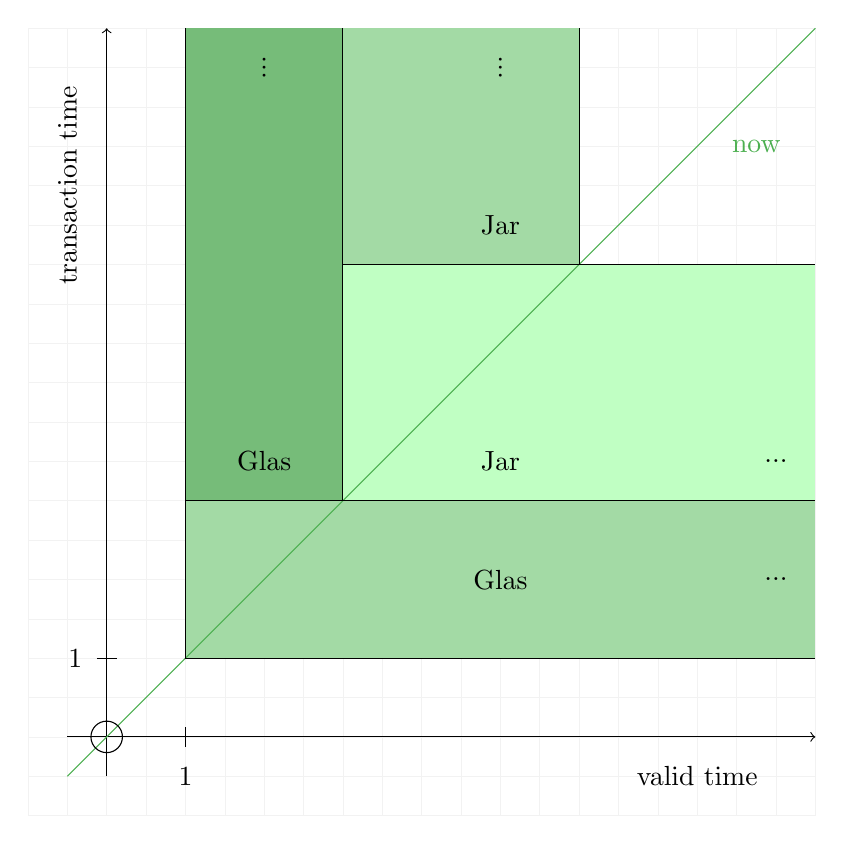
\begin{tikzpicture}
	\definecolor{brightgray}{rgb}{0.95, 0.95, 0.95}
	\definecolor{darkgreen}{RGB}{76, 175, 80}
	\definecolor{content1}{RGB}{163,218,165}
	\definecolor{content2}{RGB}{118,188,121}
	\definecolor{content3}{RGB}{192,255,195}
	
	\draw[step=.5cm,brightgray,very thin] (-1,-1) grid (9,9);
	\draw[->](-0.5, 0) -- (9,0);
	\draw[->](0, -0.5) -- (0, 9);
	\fill[content1] (1,3) -- (1,1) -- (9,1) -- (9,3);
	\fill[content2] (1,3) -- (3,3) -- (3,9) -- (1,9);
	\fill[content1] (3,9) -- (3,3) -- (6,3) -- (6,9);
	\fill[content3] (3,6) -- (3,3) -- (9,3) -- (9,6);
	
	\draw[darkgreen] (-0.5,-0.5) -- (9,9);
	\draw (0,0) circle [radius=0.2];
	\draw(-0.125, 1) -- (0.125, 1);
	\draw(1,-0.125) -- (1,0.125);
	
	\draw (1,9) -- (1,1) -- (9,1);
	\draw (1,3) -- (3,3) -- (3,9);
	\draw (3,3) -- (9,3);
	\draw (3,6) -- (6,6) -- (6,9);
	\draw (6,6) -- (9,6);
	
	\draw (-0.4, 1) node {1};
	\draw (1, -0.5) node {1};
	\draw[darkgreen](8.25,7.5) node {now};
	\draw (7.5, -0.5) node {valid time};
	\draw (-0.5, 7) node [rotate=90] {transaction time};
	
	\draw (5,2) node {Glas};
	\draw (2,3.5) node {Glas};
	\draw (5, 3.5) node {Jar};
	\draw (5,6.5) node {Jar};
	
	\draw(8.5, 2) node {...};
	\draw(2, 8.5) node [rotate=90] {...};
	\draw(8.5, 3.5) node {...};	
	\draw(5, 8.5) node [rotate=90] {...};
\end{tikzpicture}


\chapter{}
\section{Data Model}

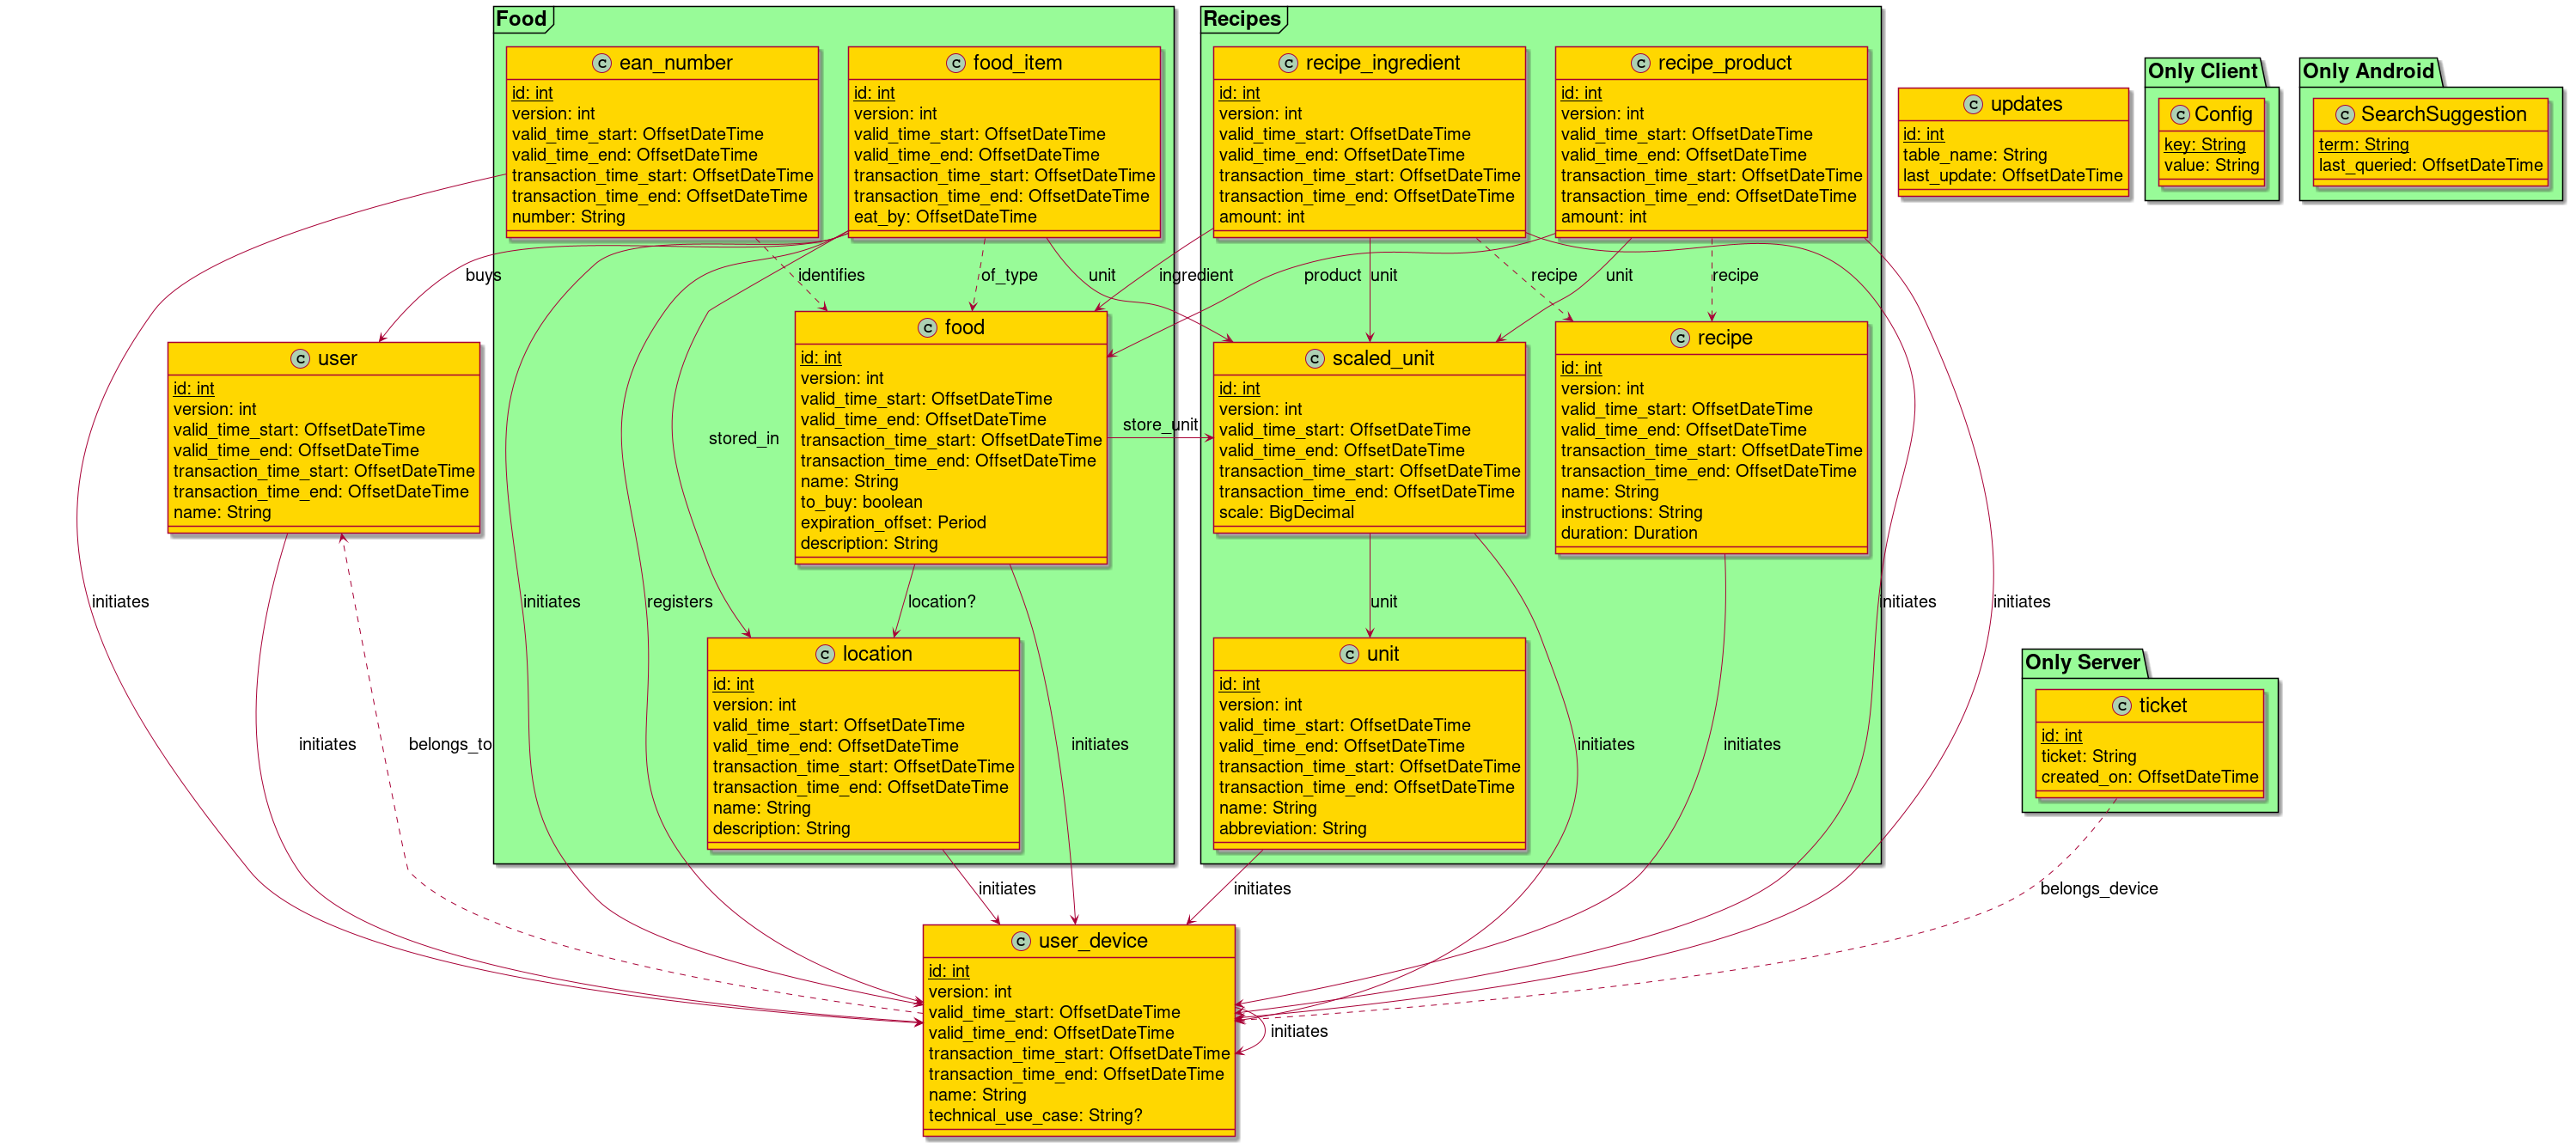
\includegraphics[width=1.25\linewidth]{diagrams/data-model.png}

\section{Architecture}

\subsection{Module Structure}

\includegraphics[width=1.25\linewidth]{diagrams/module-structure.png}

\subsection{Client}

Here interesting use cases for clients interacting with the server are described.

\paragraph{Registering a New Data Item\\}

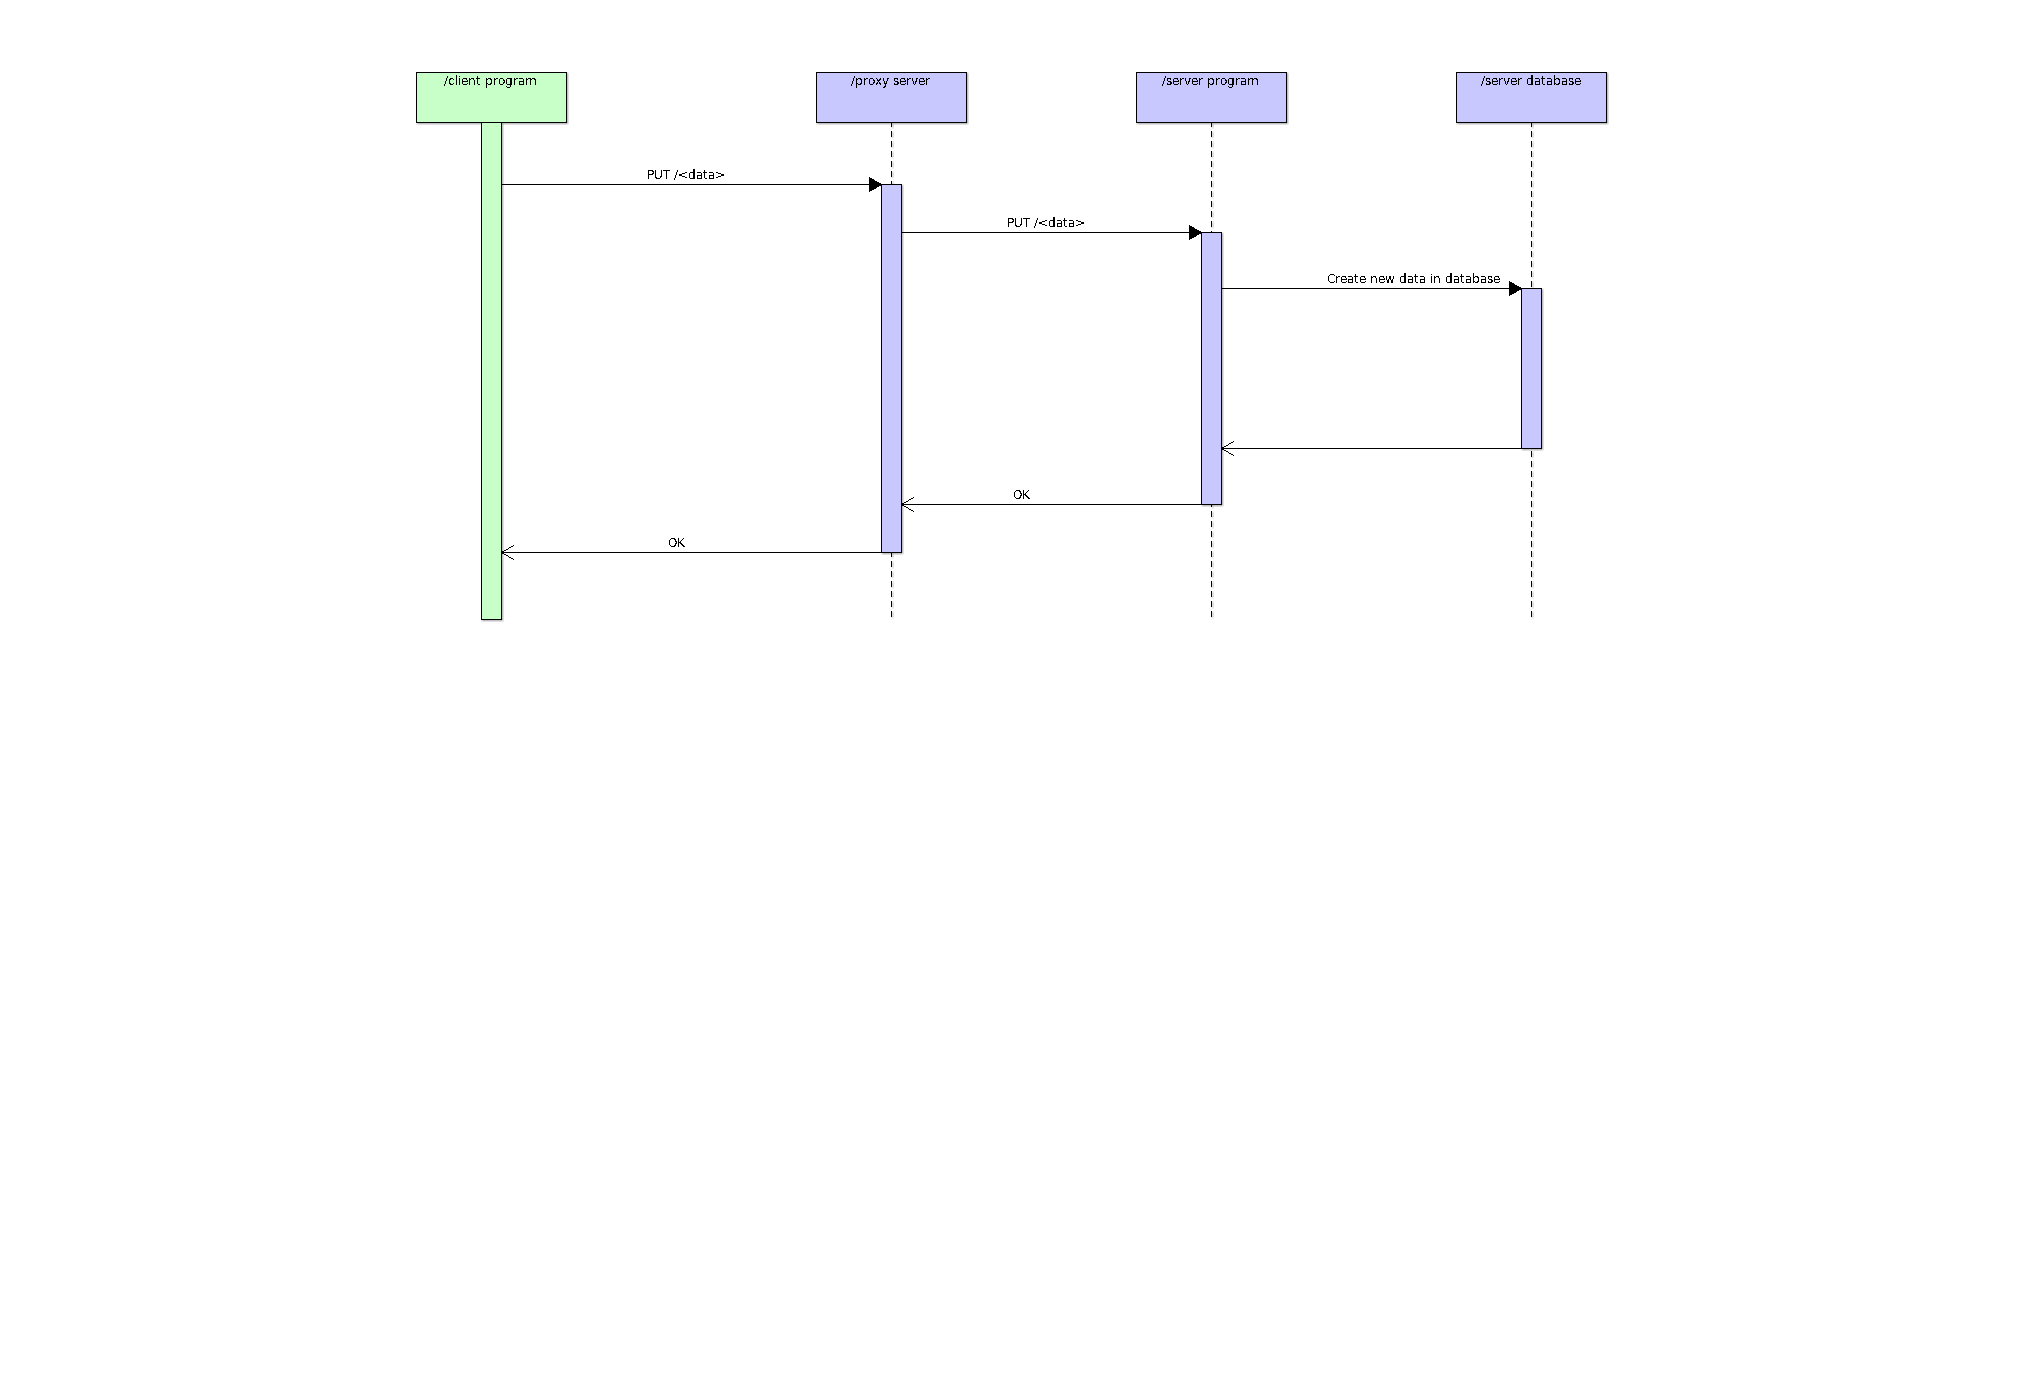
\includegraphics[width=\linewidth]{diagrams/put-data.png}

\paragraph{Refreshing the Client Database\\}

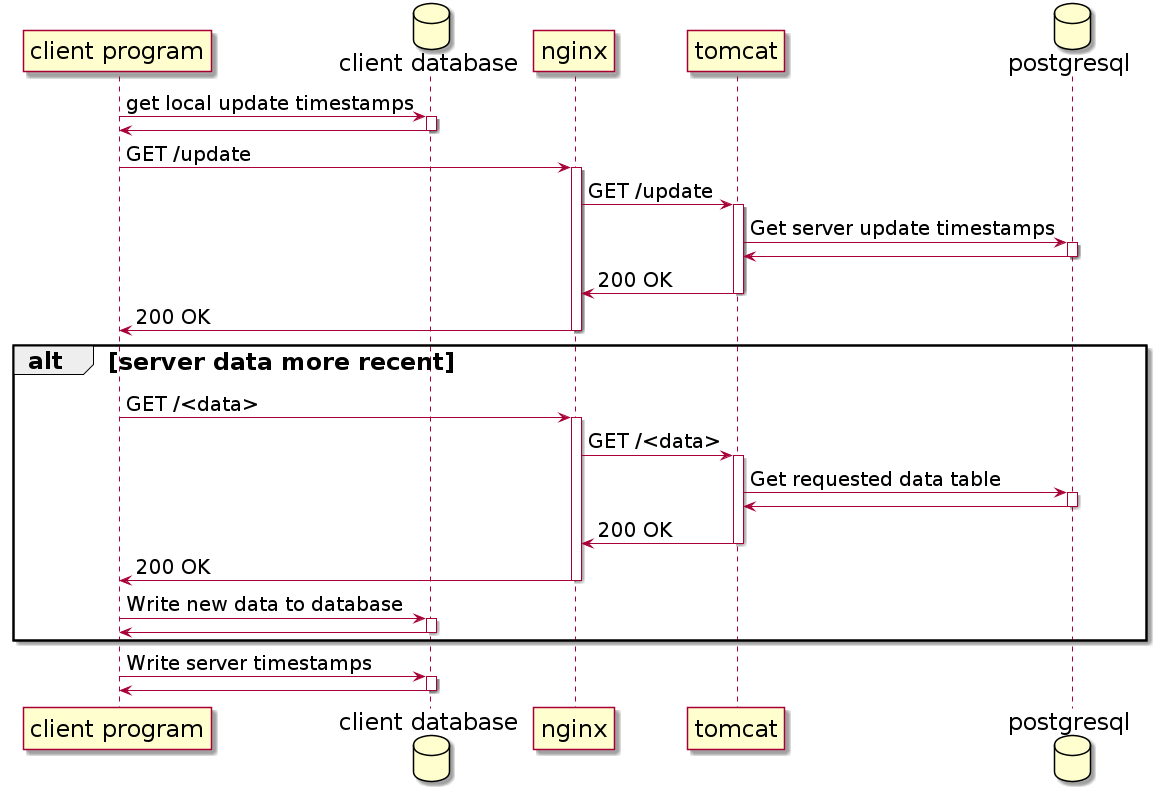
\includegraphics[width=\linewidth]{diagrams/refresh-data.png}

\paragraph{New Users' Registration}
New users are always added by giving a ticket from an existing user. The details are outlined in the diagram.

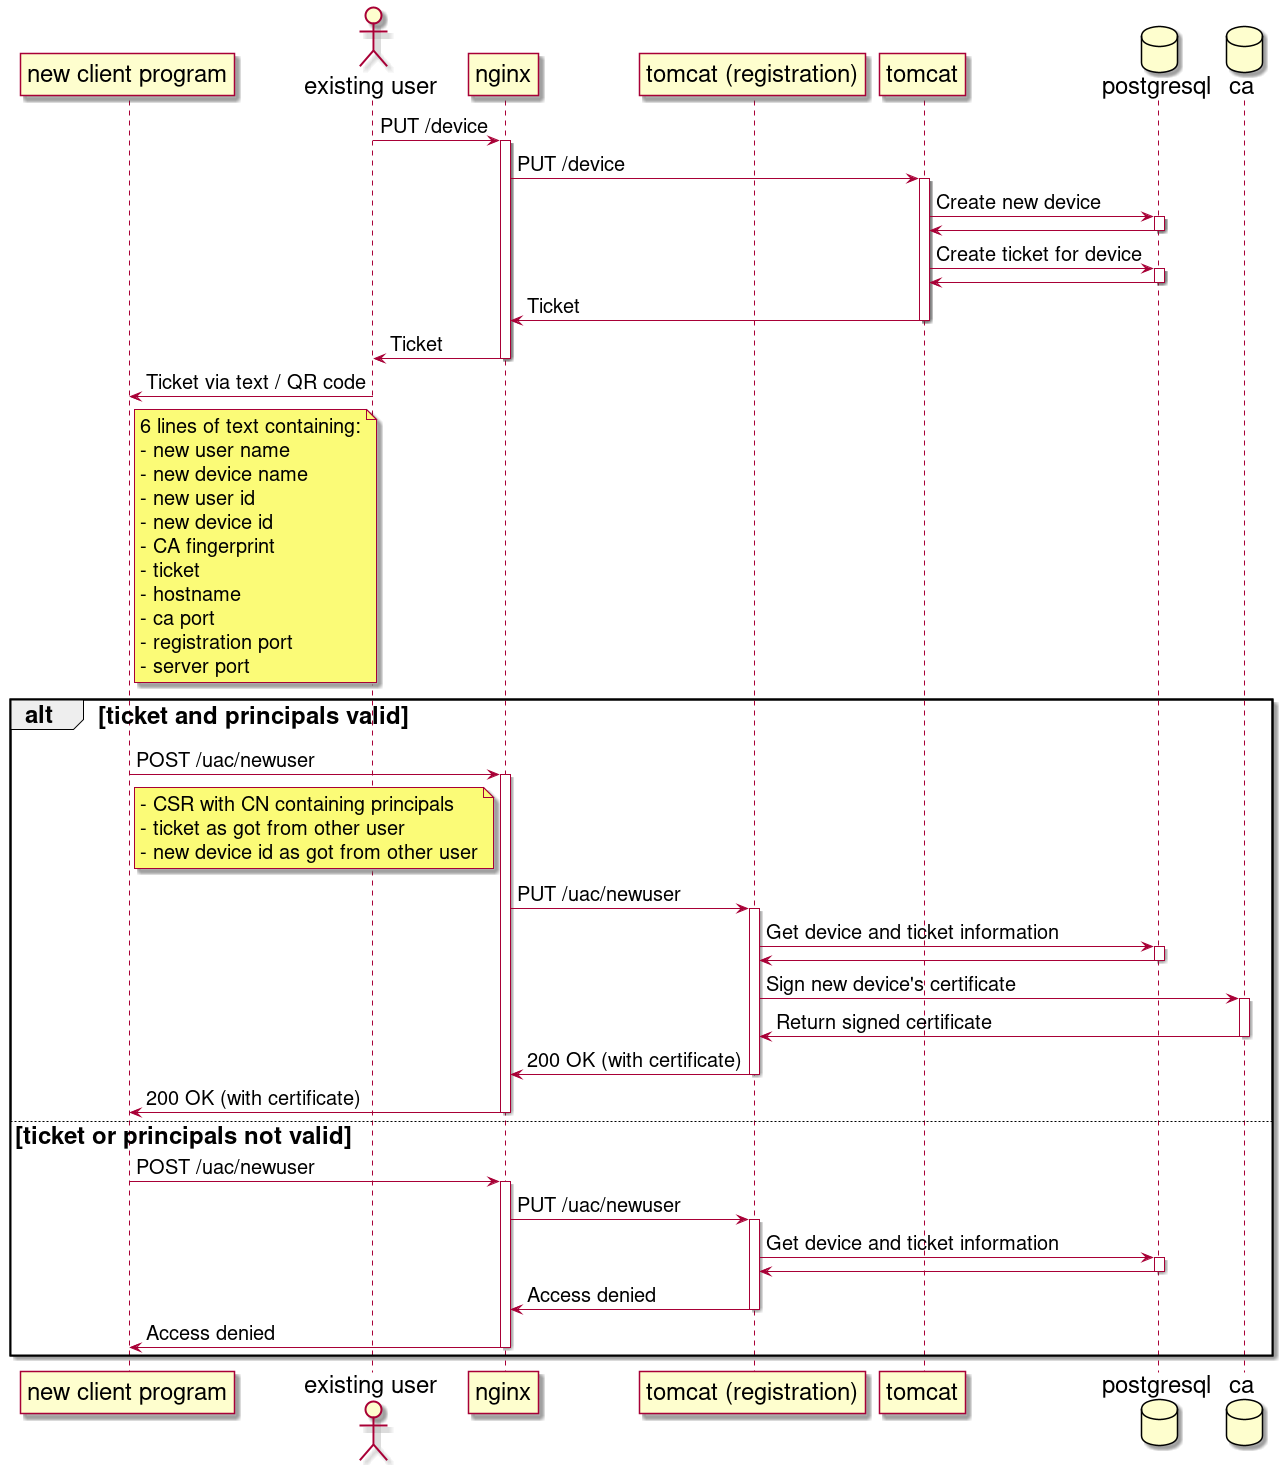
\includegraphics[width=\linewidth]{diagrams/device-registration.png}

\paragraph{Principal Names}

In the CSR the user stores the principals of his device. The values are formatted inside the Common Name attribute of the CSR. The pattern is \texttt{username \$user\_id\$devicename\$ device\_id}. So for the default test user this resolves to \texttt{Jack\$1\$Device\$1}. The principals are checked in the sentry part of the server before the certificate is signed.

\paragraph{Client Verification}

Upon receiving a new device registration request, the sentry performs the following checks in order:
\begin{itemize}
\item Check if the ticket value presented by the client is found in the database

\item Check the device id associated with the ticket from the database with the device id from the CSR

\item Check if the remaining principals of the device match the CSR

\item Check if the ticket has expired
\end{itemize}

If all the checks succeed the sentry has the CSR signed by the CA and returns it to the client.

\paragraph{QR Code Tickets}

For mobile clients it is more convenient to pass the ticket as QR code. To generate this QR code the content of the ticket has to be entered text into the QR code. The order of the values is the same as in the diagram description, i.e.

\begin{lstlisting}
Username
Device name
User ID
Device ID
CA Fingerprint
Ticket
hostname
ca port
registration port
server port
\end{lstlisting}

So for the default test user this resolves to

\begin{lstlisting}
Jack
Device
1
1
<some FPR>
0000
stocks.example
10910
10911
10912
\end{lstlisting}

\paragraph{Device Removal\\}

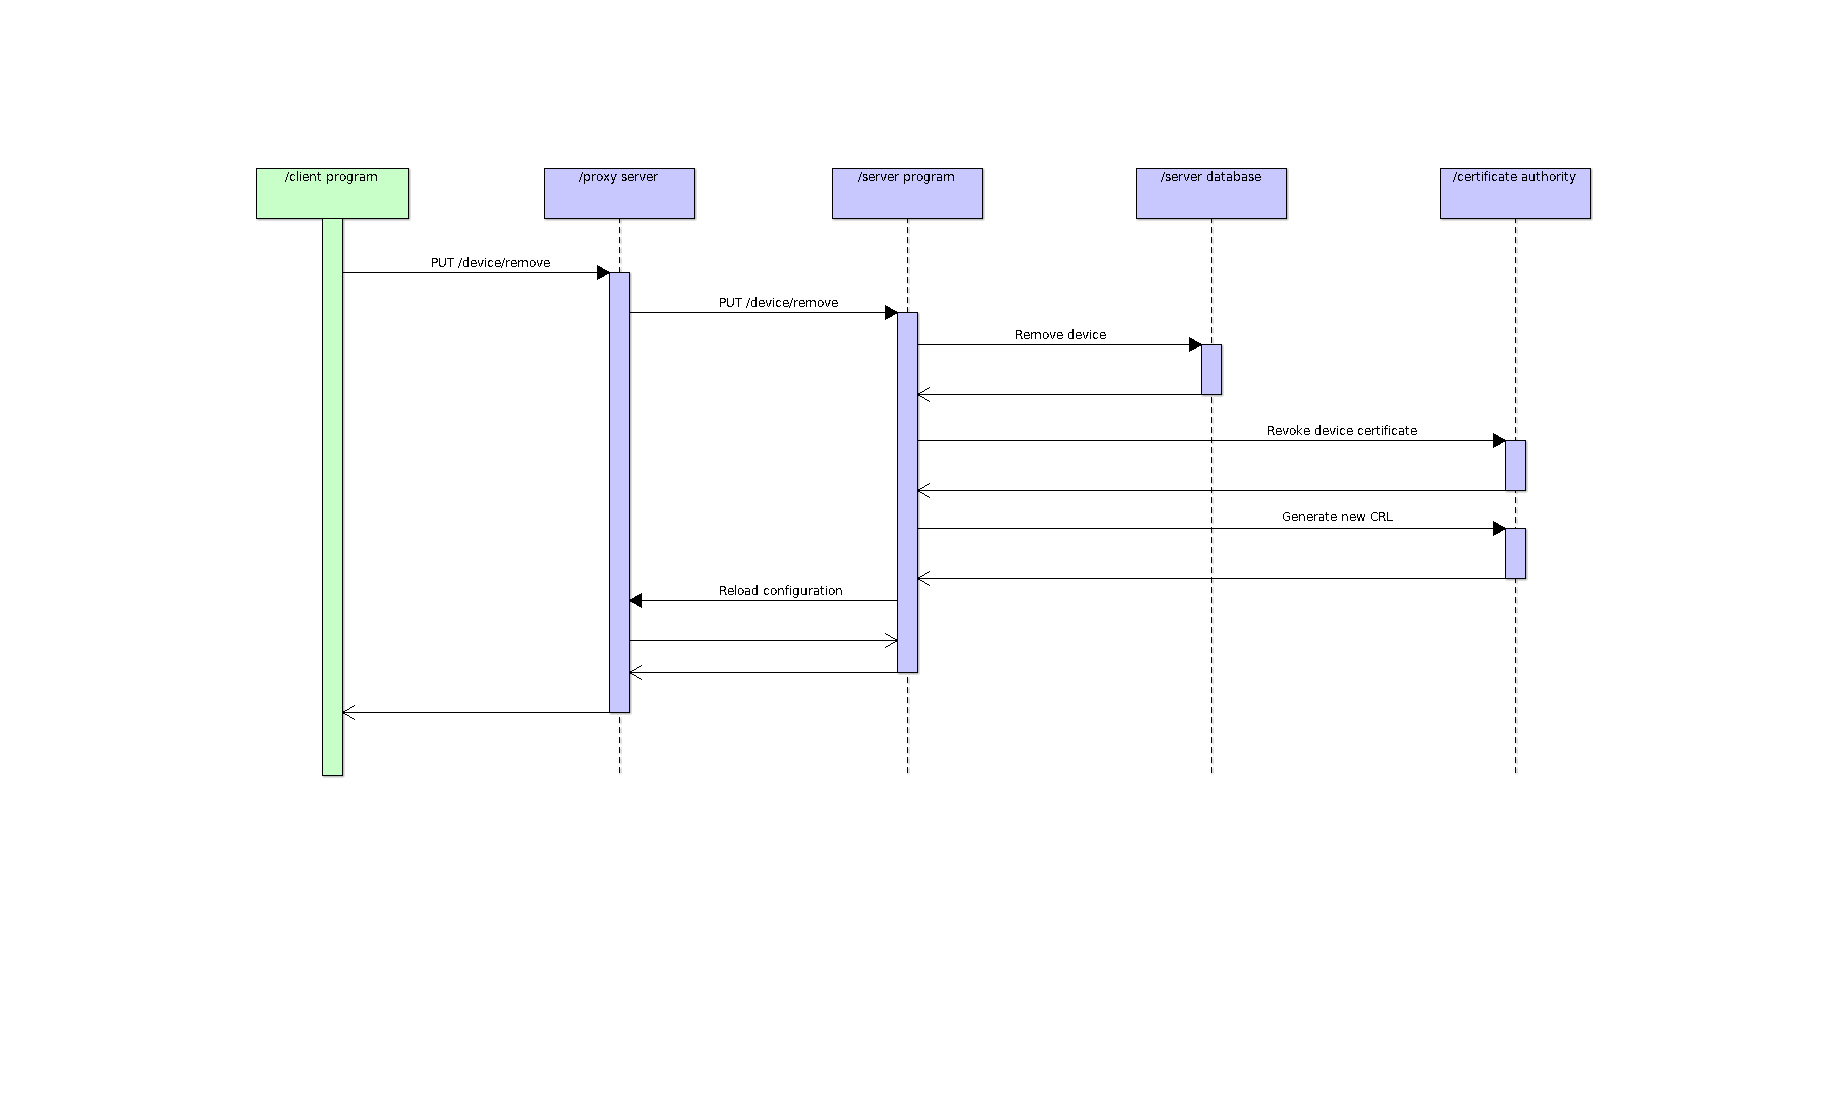
\includegraphics[width=\linewidth]{diagrams/remove-device.png}

\section{Domain Language}

\section{REST API}

Get the server's API as \href{https://spec.openapis.org/oas/latest.html}{OpenAPI specification} at \texttt{common/src/main/resources/api/openapi-spec.yaml}.

\backmatter

\end{document}